\paragraph{Exemple d'application du PFD} 

\ul{Remarque} Si $\sum \vec{F}=\vec{0}$, alors $m\vec{a}=\vec{0}$.

Choix d'une direction $\vec{i} (\overrightarrow{ox})$ \[\begin{array}{rcl}
	m\frac{d^2x}{dt^2} &=& 0 \\
	m\frac{dv}{dt} &=& 0 \\
	\frac{dv}{dt} &=& 0 \\
v(t) &=& constante \end{array}\]

$\frac{dx}{dt} = v(t) = constante = c(t) \Rightarrow x(t) = c.t + k$

Avec les conditions à \ul{t donne}, on fixe une valeur pour c et pour k.

\newpage

\subsection{Chute d'un corps près de la surface de la terre}

\begin{itemize}
	\item sans frottement
	\item mass $m_i$ ponctuelle
	\item vitesse $v_0 = 0$
	\item altitude : h
\end{itemize}

\begin{wrapfigure}[5]{r}{0pt}
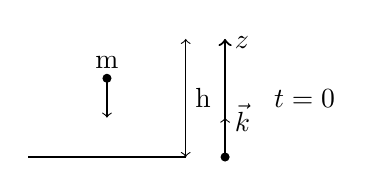
\begin{tikzpicture}
	\draw[] (-1, 0) -- (1, 0);
	\draw[->] (0, 1) -- (0, 0.5);
	\draw[fill=black] (0, 1) circle (0.05) node[yshift=0.05, above] {m};
	\node[above right] at (2, 0.5) {$t=0$};
	\draw[<->] (1, 1.5) -- (1, 0) node [midway, right] {h};
	\draw[<-, thick] (1.5, 1.5) -- (1.5, 0);
	\node[above right] at (1.5, 1.25) {$z$};
	\draw[->] (1.5, 0) -- (1.5, 0.5) node [right] {$\vec{k}$};
	\draw[fill=black] (1.5, 0) circle (0.05);
\end{tikzpicture}
\end{wrapfigure}

\[\begin{array}{rclr}
	\text{Bilan des forces} &=& \vec{P} \\
					&=& m\vec{g} & ||\vec{g}||=g \\
		\vec{P} &=& -mg\vec{k}\end{array}\]

PFD: $\sum\vec{F} = m\vec{a} = \vec{P} = -mg\vec{k} $
\[ \text{Equations différentielles du mouvement : ~\\
	derive seconde }\left\{ \begin{array}{rcl}
	m\ddot{x} &=& 0 \\
	m\ddot{y} &=& 0 \\
m\ddot{z} &=& -mg \end{array} \right. \]

\ul{Solution des equations differentielles} : ~\\
\[\text{derive premiere } \left\{ \begin{array}{rcl}
			\dot{x} &=&C_1 \\
			\dot{y} &=&C_2 \\
			\dot{z} &=& -mg
		\end{array}\right. \left\{\begin{array}{rclr}
			\ddot{z} &=& -g \\
		\dot{z} &=& -gt + C_z & \text{ On passe par la primitive} \end{array}\right.
\]

\[\text{pour } t=0 \text{ } \vec{v} \left\{ \begin{array}{rcl}
			\dot{x}(0) &=&0 \\
			\dot{y}(0) &=&0 \\
	\dot{z}(0) &=&0 \end{array}\right.\] 

			On remplace pour $t=0$ : ~\\
			$\dot{x}(0) = C_1 = 0$ ~\\
			$\dot{y}(0) = C_2 = 0$ ~\\
			$\dot{z}(0) = (-gt+C_3) = C_3 = 0$
			
			\[\text{Donc : } \vec{v} \left\{ \begin{array}{rcl} 
			\dot{x}(t) &=&0 \\
			\dot{y}(t) &=&0 \\
			\dot{z}(t) &=& -gt \end{array} \right. \]

\subsection{Chute d'un corps dans un fluide} ~\\
Les positions à chaque \ul{t} : \[\left\{ \begin{array}{r}
			x(t) \\
			y(t) \\
		z(t) \end{array} \right.
		\text{Les primitives de } \dot{x}, \dot{y}, \dot{z} \Rightarrow \left\{ \begin{array}{rcl}
			x(t) &=& C_x \\
			y(t) &=& C_y \\
			z(t) &=& \int{-gt dt} = -\frac{g}{2}t^2 + C_z \end{array} \right. \]

		\[\text{ pour } t=0 \left\{ \begin{array}{rcl}
					x(0)&=&0 \Rightarrow C_x = 0 \\
					y(0)&=&0 \Rightarrow C_y = 0\\
					z(0)&=&h \Rightarrow C_z = h
			\end{array} \right. \]

	\paragraph{Exemples d'application du PFD}
			\begin{wrapfigure}[5]{r}{0pt}
				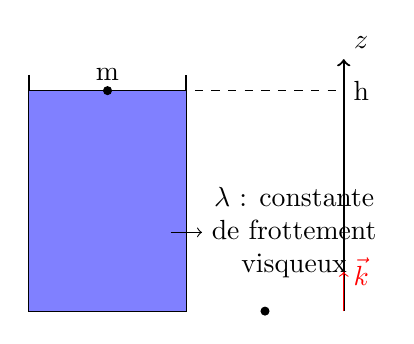
\begin{tikzpicture}
					\draw[thick] (-1, 3) -- (-1, 0) -- (1, 0) -- (1, 3);
					\draw[fill=blue!50] (-1, 2.8) -- (-1, 0) -- (1, 0) -- (1, 2.8) -- cycle;
					\draw[->] (0.8, 1) -- (1.2, 1) node [right, align=center] {$\lambda$ : constante \\
					de frottement\\
					visqueux};
					\draw[->, thick] (3, 0) -- (3, 3.2) node [above right] {$z$};
					\draw[dashed] (-1, 2.8) -- (3, 2.8) node [right] {h};
					\draw[fill=black] (0, 2.8) circle (0.05) node [above] {m};
					\draw[red, ->] (3, 0) -- (3, 0.5) node [right] {$\vec{k}$};
					\draw[fill = black] (2, 0) circle (0.05);
				\end{tikzpicture}
			\end{wrapfigure}

			\begin{itemize}
				\item m : ponctuelle. \[t=0 \left\{ \begin{array}{rcl} z&=&h \\
			v &=& 0 \end{array}\right. \]
				\item Bilan des forces : $\vec{P} = m\vec{g}$, force de frottement visqueux / fluide : $\vec{f} = -\lambda \vec{v}$
				\item PFD : \[\begin{array}{rclr}
							m\vec{a} &=& \vec{P} + \vec{f} \\
								   &=& -mg\vec{k} - \lambda \vec{v} & ||\vec{g}|| = g \\
								   &=& -mg\vec{k} - \lambda v\vec{k} & v \left\{ \begin{array}{c}
															\dot{x} \\
															\dot{y} \\
														\dot{z} \end{array} \right.
					\end{array}\] \[\left\{\begin{array}{rcl}
								m\ddot{x} &=&0 \\
								m\ddot{y} &=&0 \\
						m\ddot{z} &=& -mg-\lambda \dot{z} \end{array} \right.
								\left\{\begin{array}{rclr}
									m\dot{v}_x &=& 0 \\
									m\dot{v}_y &=& 0 \\
									m\dot{v}_z &=& -mg - \lambda v_z &(3) \end{array} \right. \Rightarrow \left\{\begin{array}{rcl}
										v_x &=& C_x \\
										v_y &=& C_y
								\end{array}\right.\]
								~\\

$(3) \text{ } \dot{v}_z + \frac{\lambda}{m}v_z = -g$ ~\\
~\\
On pose : $\frac{\lambda}{m} = \frac{1}{\tau} \Rightarrow \dot{v}_z + \frac{v_z}{\tau} = -g (3)'$ 
			\end{itemize}
			~\\

La solution de $(3)'$ est la solution de l'équation sans second membre (ou équation homogène) ~\\
				\fbox{$\dot{v}_z + \frac{v_z}{\tau} = 0$} (équation homogène) + Une \ul{Solution particuliere} de $(3)$ ~\\
				\[\begin{array}{rcl}
					V_z &=& V_z^{(P)} + V_z^{(H)}
				\end{array}\]
				~\\

La solution de l'équation Homogène : ~\\
	$\dot{v}_z + \frac{v_z}{\tau} = 0$ est de la forme : ~\\
	\begin{center}
	\fbox{$v_z^H(t) = K * e^{-\frac{t}{\tau}}$}
	\end{center}
	~\\

	La solution particulière est de la même forme que le $2^{nd}$ membre donc \[\begin{array}{rcl}
			V_z^{(P)} &=& constante \\
	\dot{V}_z^{(P)} &=& 0 \end{array}\]

			On remplace dans (3)' : 
			$0 + \frac{V_z^P}{\tau} = -g \Rightarrow v_z^{(P)} = -g\tau$ 

			Donc la solution de l'équation différentielle de $(3)$ est :

			\begin{center}
				\fbox{$v_z(t) = V_z^H + v_z^P = Ke^{-\frac{t}{\tau}} -g\cdot \tau$}
			\end{center}

			à $t=0$ $v_z=0$
			\[\begin{array}{rcl}
					v_z(0) &=& K * (1) - g\tau = 0 \\
					K &=& g\tau \Rightarrow \begin{array}{rcl} 
						v_z(t) &=&  g \tau e^{-\frac{t}{\tau}} - g \tau \\
						&=& -g\tau[1-e^{-\frac{t}{\tau}}] \end{array}
			\end{array} \]

			à $t=0$, $e^{-\frac{1}{\tau}} = 1$ et $v_z=0$ ~\\
			~\\
			Pour $t >> \tau$, alors $\begin{array}{rcl}
				e^{-\frac{t}{\tau}} &\rightarrow& 0 \\
				v_z & \rightarrow -g\tau \end{array}$

			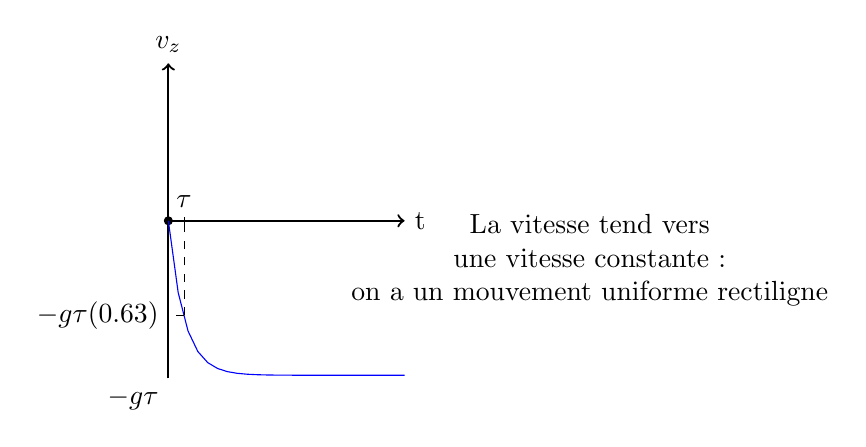
\begin{tikzpicture}
				\draw[fill=black] (0, 0) circle (0.05);
				\draw[thick, ->] (0, 0) -- (3, 0) node [right] {t};
				\draw[thick, ->] (0, -2) -- (0, 2) node [above] {$v_z$};
				\draw[blue, domain=0:3] plot(\x, {-9.81*0.2 * (1-exp(-\x / 0.2))});

				\draw[] (0.2, -0.05) -- (0.2, 0.05) node [above] {$\tau$};
				\draw[dashed] (0.2, -1.2) -- (0.2, 0);
				\draw[dashed] (0.2, -1.2) -- (0, -1.2) node [left] {$-g\tau(0.63)$};
				\node[below left] at (0, -2) {$-g\tau$};
				\node[right, align=center] at (2.2, -0.5) {La vitesse tend vers \\ une vitesse constante : \\ on a un mouvement uniforme rectiligne};
			\end{tikzpicture}

			\paragraph{Calcul de z(t)}

			\[\begin{array}{rcl}
					v_z(t) &=& \dot{z}(t) \\
					z(t) &=& \int{\dot{z}(t)} = \int{[-g\tau (1-e^{-\frac{t}{\tau}})]dt} \\
							   &=& \int{[(-g\tau)dt + (g\tau e^{-\frac{t}{\tau}})]dt} \\
							   &=& -g\tau \cdot t + g\tau\int{e^{-\frac{t}{\tau}} dt} + g\tau(-\cfrac{1}{\cfrac{1}{\tau}})e^{-\frac{t}{\tau}}+K_z \\
							   &=& -g\tau t - g\tau^2 e^{-\frac{t}{\tau}} + K_z \\
						 &=& -g\tau ^2 [\frac{t}{\tau}+ e^{-\frac{t}{\tau}}] + K_z
			\end{array}\]
		

			à $t=0$, $z(0)=h$ ~\\
			~\\
			$z(0) = 0 - g\tau ^2*1+K_z = h$ ~\\
			$K_z = h+g\tau ^2$

			\begin{center}

			On remplace dans $(4)$: ~\\
			$z(t) = -g\tau ^2 [\frac{t}{\tau}+e^{-\frac{t}{\tau}}]+h+g\tau ^2$

			\fbox{$z(t) = h - g\tau ^2[\frac{t}{\tau} + e^{-\frac{t}{\tau}}-1]$}
		\end{center}
